\subsection{区间估计}\label{sec:10.4}
像前两节一样，现在探讨置信集的若干近似和渐近版本. 目的仍是说明一些在更复杂情形中有用、能够得到某种答案的方法. 这里所得的答案几乎肯定不是最好的，但也肯定不是最坏的. 不过，在许多情形下，它们是我们所能做到的最好结果.

与前面一样，从基于MLE的近似开始.

\subsubsection{近似最大似然区间}\label{sec:10.4.1}
由\autoref{sec:10.1.2}的讨论，使用\autoref{thm:10.1.12}，有一般方法求得MLE的渐近分布. 因而也有一般方法构造置信区间.

若$X_1,\ldots,X_n$独立同分布于$f(x\mid\theta)$，$\hat\theta$是$\theta$的MLE，则由\hyperref[eq:10.1.7]{(7.4.1)}，函数$h(\hat\theta)$的方差可近似为\footnote{译注：原文引用公式(7.4.1)，但与下式直接对应的是\eqref{eq:10.1.7}. 保留原引用，待对照作者勘误核实.}
$$\widehat{\operatorname{Var}}(h(\hat\theta)\mid\theta)\approx\frac{[h'(\theta)]^2|_{\theta=\hat\theta}}{-\frac{\partial^2}{\partial\theta^2}\log L(\theta\mid\boldsymbol x)|_{\theta=\hat\theta}}.$$

\sourcepageanchor{433}
现在，对固定但任意的$\theta$，关心
$$\frac{h(\hat\theta)-h(\theta)}{\sqrt{\widehat{\operatorname{Var}}(h(\hat\theta)\mid\theta)}}$$
的渐近分布. 由\autoref{thm:10.1.12}及Slutsky定理（\autoref{thm:5.5.17}；见\autoref{exercise:10.33}），
$$\frac{h(\hat\theta)-h(\theta)}{\sqrt{\widehat{\operatorname{Var}}(h(\hat\theta)\mid\theta)}}\longrightarrow\mathrm n(0,1),$$
从而给出近似置信区间
$$h(\hat\theta)-z_{\alpha/2}\sqrt{\widehat{\operatorname{Var}}(h(\hat\theta)\mid\theta)}\leq h(\theta)\leq h(\hat\theta)+z_{\alpha/2}\sqrt{\widehat{\operatorname{Var}}(h(\hat\theta)\mid\theta)}.$$

\begin{example}[续\autoref{ex:10.1.14}]\label{ex:10.4.1}\index{SI0138@二项}
设$X_1,\ldots,X_n$为Bernoulli$(p)$总体的随机样本. 已经看到，可以用MLE $\hat p/(1-\hat p)$估计优势比$p/(1-p)$，且这个估计的近似方差为
$$\widehat{\operatorname{Var}}\left(\frac{\hat p}{1-\hat p}\right)\approx\frac{\hat p}{n(1-\hat p)^3}.$$
因此，可以构造近似置信区间
$$\frac{\hat p}{1-\hat p}-z_{\alpha/2}\sqrt{\widehat{\operatorname{Var}}\left(\frac{\hat p}{1-\hat p}\right)}
\leq\frac p{1-p}\leq\frac{\hat p}{1-\hat p}+z_{\alpha/2}\sqrt{\widehat{\operatorname{Var}}\left(\frac{\hat p}{1-\hat p}\right)}.$$
\end{example}

一种限制较多的似然近似形式基于得分统计量（\autoref{sec:10.3.2}）；但在适用时，它能给出更好的区间. 随机量
\begin{equation}\label{eq:10.4.1}
Q(\boldsymbol X\mid\theta)=\frac{\frac\partial{\partial\theta}\log L(\theta\mid\boldsymbol X)}{\sqrt{-E_\theta\left(\frac{\partial^2}{\partial\theta^2}\log L(\theta\mid\boldsymbol X)\right)}}
\end{equation}
在$n\to\infty$时渐近服从$\mathrm n(0,1)$分布. 因此集合
\begin{equation}\label{eq:10.4.2}\index{SI0139@最大似然}
\{\theta:|Q(\boldsymbol x\mid\theta)|\leq z_{\alpha/2}\}
\end{equation}
是近似$1-\alpha$置信集. 注意，应用\autoref{sec:7.3.2}的结果，有
$$E_\theta(Q(\boldsymbol X\mid\theta))=\frac{E_\theta\left(\frac\partial{\partial\theta}\log L(\theta\mid\boldsymbol X)\right)}{\sqrt{-E_\theta\left(\frac{\partial^2}{\partial\theta^2}\log L(\theta\mid\boldsymbol X)\right)}}=0,$$
且
\begin{equation}\label{eq:10.4.3}
\operatorname{Var}_\theta(Q(\boldsymbol X\mid\theta))=\frac{\operatorname{Var}_\theta\left(\frac\partial{\partial\theta}\log L(\theta\mid\boldsymbol X)\right)}{-E_\theta\left(\frac{\partial^2}{\partial\theta^2}\log L(\theta\mid\boldsymbol X)\right)}=1.
\end{equation}
所以这个近似精确匹配$\mathrm n(0,1)$随机变量的前两阶矩. \hyperref[bib:source330]{Wilks（1938）}证明，这些区间具有渐近最优性：渐近地，它们是某类区间中最短的.

当然，这些区间并非完全一般，未必总能适用于函数$h(\theta)$. 必须能够把\eqref{eq:10.4.2}表示为$h(\theta)$的函数.

\sourcepageanchor{434}
\begin{example}[二项得分区间]\label{ex:10.4.2}
再次使用二项例子，若$Y=\sum_{i=1}^nX_i$，每个$X_i$都是独立的Bernoulli$(p)$随机变量，则有
$$\begin{aligned}
Q(Y\mid p)&=\frac{\frac\partial{\partial p}\log L(p\mid Y)}{\sqrt{-E_p\left(\frac{\partial^2}{\partial p^2}\log L(p\mid Y)\right)}}\\
&=\frac{\frac yp-\frac{n-y}{1-p}}{\sqrt{\frac n{p(1-p)}}}
=\frac{\hat p-p}{\sqrt{p(1-p)/n}},
\end{aligned}$$
其中$\hat p=y/n$. 利用\eqref{eq:10.4.2}，得到近似$1-\alpha$置信区间
\begin{equation}\label{eq:10.4.4}
\left\{p:\left|\frac{\hat p-p}{\sqrt{p(1-p)/n}}\right|\leq z_{\alpha/2}\right\}.
\end{equation}
这是反演得分统计量（\autoref{ex:10.3.6}）所得的区间. 计算它需要解一个关于$p$的二次方程，细节见\autoref{ex:10.4.6}.
\end{example}

在\autoref{sec:10.3}中，根据$-2\log\lambda(\boldsymbol X)$渐近服从卡方分布这一事实，导出了另一种似然检验. 这提示：若$X_1,\ldots,X_n$独立同分布于$f(x\mid\theta)$，$\hat\theta$是$\theta$的MLE，则集合
\begin{equation}\label{eq:10.4.5}
\left\{\theta:-2\log\left(\frac{L(\theta\mid\boldsymbol x)}{L(\hat\theta\mid\boldsymbol x)}\right)\leq\chi_{1,\alpha}^2\right\}
\end{equation}
是近似$1-\alpha$置信区间. 确实如此，这又给出了一个近似似然区间.

当然，\eqref{eq:10.4.5}就是最初通过反演LRT统计量导出的最高似然区域\eqref{eq:9.2.7}. 不过，现在有了自动赋予近似置信水平的方法.

\begin{example}[二项LRT区间]\label{ex:10.4.3}
若$Y=\sum_{i=1}^nX_i$，每个$X_i$都是独立的Bernoulli$(p)$随机变量，则近似$1-\alpha$置信集为
$$\left\{p:-2\log\left(\frac{p^y(1-p)^{n-y}}{\hat p^y(1-\hat p)^{n-y}}\right)\leq\chi_{1,\alpha}^2\right\}.$$
\autoref{ex:10.4.7}将比较这个置信集与基于得分检验和Wald检验的区间.
\end{example}

\subsubsection{其他大样本区间}\label{sec:10.4.2}
多数近似置信区间基于寻找近似（或渐近）枢轴量，或者反演近似水平$\alpha$的检验统计量. 若有任意统计量$W$、$V$与参数$\theta$，使$n\to\infty$时
$$\frac{W-\theta}V\longrightarrow\mathrm n(0,1),$$
则可以构造$\theta$的近似置信区间
$$W-z_{\alpha/2}V\leq\theta\leq W+z_{\alpha/2}V,$$
本质上是Wald型区间. 直接应用中心极限定理与Slutsky定理，通常就会给出近似置信区间. （注意，上一小节的近似最大似然区间均体现这一策略.）

\sourcepageanchor{435}
\begin{example}[近似区间]\label{ex:10.4.4}\index{SI0137@近似}
若$X_1,\ldots,X_n$独立同分布，均值为$\mu$、方差为$\sigma^2$，则由中心极限定理，
$$\frac{\bar X-\mu}{\sigma/\sqrt n}\longrightarrow\mathrm n(0,1).$$
此外，由Slutsky定理，若$S^2$依概率收敛到$\sigma^2$，则
$$\frac{\bar X-\mu}{S/\sqrt n}\longrightarrow\mathrm n(0,1),$$
给出近似$1-\alpha$置信区间
\begin{equation}\label{eq:10.4.6}
\bar x-z_{\alpha/2}s/\sqrt n\leq\mu\leq\bar x+z_{\alpha/2}s/\sqrt n.
\end{equation}
为了解近似有多好，对多种pdf进行小型模拟，计算近似区间的精确覆盖概率. 注意，因为区间基于枢轴量，覆盖概率不依赖参数值；它是常数，因此就是置信系数. \autoref{tab:10.4.7}显示，即使样本量小至$n=15$，枢轴置信区间也有合理表现，但显然达不到名义置信系数. 这无疑是由于使用$z_{\alpha/2}$临界值过于乐观，没有计入$S$的变动. 样本量增大时，近似将改善.

\par\begin{table}[htbp]\centering\setcounter{table}{6}
\caption{枢轴区间\eqref{eq:10.4.6}的置信系数，$n=15$，基于10,000次模拟}\label{tab:10.4.7}
\begin{tabular}{l|rrrr}\toprule
&\multicolumn{4}{c}{基础pdf}\\\cmidrule(lr){2-5}
名义水平&正态&$t_5$&逻辑斯蒂&双指数\\\midrule
$1-\alpha=.90$&0.879&0.864&0.880&0.876\\
$1-\alpha=.95$&0.931&0.924&0.931&0.933\\\bottomrule
\end{tabular}
\end{table}\par
\end{example}

上例无需指定抽样分布形式，就能得到近似置信区间. 当指定分布形式时，应能做得更好.

\begin{example}[近似泊松区间]\label{ex:10.4.5}\index{SI0141@泊松}
若$X_1,\ldots,X_n$独立同分布于Poisson$(\lambda)$，则知道
$$\frac{\bar X-\lambda}{S/\sqrt n}\longrightarrow\mathrm n(0,1).$$
不过，即使不是从泊松总体抽样，这也成立. 利用泊松假设，知道$\operatorname{Var}(X)=\lambda=EX$，且$\bar X$是$\lambda$的良好估计量（\autoref{sec:7}）. 因此利用泊松假设，还能由
$$\frac{\bar X-\lambda}{\sqrt{\bar X/n}}\longrightarrow\mathrm n(0,1)$$
得到近似置信区间，它是反演Wald检验所得的区间. 还可以用另一种方式利用泊松假设. 因为$\operatorname{Var}(X)=\lambda$，所以
$$\frac{\bar X-\lambda}{\sqrt{\lambda/n}}\longrightarrow\mathrm n(0,1),$$
由此得到与得分检验对应的区间，也就是\eqref{eq:10.4.2}的似然区间；按\hyperref[bib:source330]{Wilks（1938）}的结果，它是最优的（见\autoref{exercise:10.40}）.
\end{example}

\sourcepageanchor{436}
一般而言，合理的经验法则是，在近似中尽可能少用估计值、多用参数. 理由很简单：参数固定，不给近似引入额外变动，而每个统计量都会带来更多变动.

\begin{example}[再论二项得分区间]\label{ex:10.4.6}
对Bernoulli$(p)$总体的随机样本$X_1,\ldots,X_n$，在\autoref{ex:10.3.5}中看到，当$n\to\infty$时，
$$\frac{\hat p-p}{\sqrt{\hat p(1-\hat p)/n}}\quad\text{与}\quad\frac{\hat p-p}{\sqrt{p(1-p)/n}}$$
均依分布收敛到标准正态随机变量，其中$\hat p=\sum x_i/n$. 在\autoref{ex:10.3.5}中看到，可以基于任一近似建立检验，前者为Wald检验，后者为得分检验. 也知道可以用任一近似构造$p$的置信区间. 不过，得分检验近似使用较少的统计量和较多的参数值，会给出\autoref{ex:10.4.2}中的区间\eqref{eq:10.4.4}，它是渐近最优的. 即
$$\left\{p:\left|\frac{\hat p-p}{\sqrt{p(1-p)/n}}\right|\leq z_{\alpha/2}\right\}$$
是更好的近似区间.

这个区间的样子并不一目了然，但可以显式解出其取值集合. 两边平方并整理，就要寻找满足
$$\left\{p:(\hat p-p)^2\leq z_{\alpha/2}^2\frac{p(1-p)}n\right\}$$
的$p$值. 这是关于$p$的二次不等式，进一步整理可写成熟悉的形式：
$$\left\{p:\left(1+\frac{z_{\alpha/2}^2}n\right)p^2-\left(2\hat p+\frac{z_{\alpha/2}^2}n\right)p+\hat p^2\leq0\right\}.$$
由于二次项系数为正，抛物线开口向上，因此当$p$位于两个根之间时不等式成立. 两个根为
\begin{equation}\label{eq:10.4.7}
\frac{2\hat p+z_{\alpha/2}^2/n\ \pm\sqrt{(2\hat p+z_{\alpha/2}^2/n)^2-4\hat p^2(1+z_{\alpha/2}^2/n)}}{2(1+z_{\alpha/2}^2/n)},
\end{equation}
它们定义$p$的置信区间端点. 虽然根的表达式有些繁琐，这实际上是$p$的一个很好区间. 不过，使用连续性校正（\autoref{ex:3.3.2}）还可进一步改进. 为此，需要分别解两个二次不等式（见\autoref{exercise:10.45}）：
$$\begin{aligned}
\left|\frac{\hat p+\frac1{2n}-p}{\sqrt{p(1-p)/n}}\right|&\leq z_{\alpha/2},&&\text{（较大根为区间上端点）},\\
\left|\frac{\hat p-\frac1{2n}-p}{\sqrt{p(1-p)/n}}\right|&\leq z_{\alpha/2}.&&\text{（较小根为区间下端点）}.
\end{aligned}$$
在端点处有显然的修正：若$\sum x_i=0$，则区间下端点取0；若$\sum x_i=n$，则区间上端点取1. 一些良好近似见\hyperref[bib:source39]{Blyth（1986）}.
\end{example}

\sourcepageanchor{437}
现在已经看到二项比例的三个区间：基于Wald统计量、得分统计量的区间，以及\autoref{ex:10.4.3}的LRT区间. 通常最不优先选择Wald区间，不过比较三者仍很有意思.

\begin{example}[二项区间的比较]\label{ex:10.4.7}
对$Y=\sum_{i=1}^nX_i$，其中$X_1,\ldots,X_n$独立同分布于Bernoulli$(p)$总体，Wald区间为
\begin{equation}\label{eq:10.4.8}
\hat p-z_{\alpha/2}\sqrt{\frac{\hat p(1-\hat p)}n}\leq p\leq\hat p+z_{\alpha/2}\sqrt{\frac{\hat p(1-\hat p)}n}.
\end{equation}
带连续性校正的得分区间见\autoref{ex:10.4.6}，近似LRT见\autoref{ex:10.4.3}. 为比较它们，来看一个例子.

\par\begin{figure}[htbp]\centering
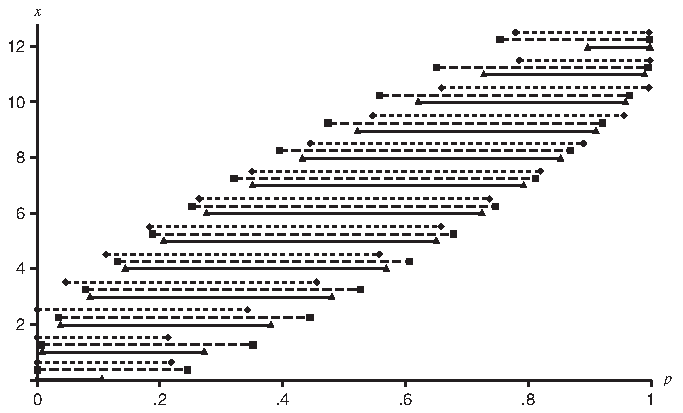
\includegraphics[width=.9\textwidth]{assets/chapter10/fig-10.4.1.pdf}
\caption{LRT程序（实线）、得分程序（长虚线）和修正Wald程序（短虚线）给出的二项比例区间.}\label{fig:10.4.1}
\end{figure}\par

对$n=12$，\autoref{fig:10.4.1}显示三种程序的区间实现值. LRT程序给出的区间最短，得分区间最长. 在这幅图中，对Wald区间作了两项修正. 首先，当$y=0$时，未修正区间为$(0,0)$，故将上端点改为$1-(\alpha/2)^{1/n}$；在$y=n$时对下端点作相似修正. 另外，Wald区间端点有时会超出$[0,1]$，这些部分已被截断.

得分区间较长，反映在其覆盖概率更高. 实际上，三者中只有得分区间保持覆盖概率在$.9$以上，因此只有它的置信系数为$.9$. LRT与Wald区间似乎太短，覆盖概率远低于$.9$，难以接受. 当然，随着$n$增大，它们的表现会改善. 其他选择见\hyperref[sec:9.5.2]{杂录9.5.2}.

所以，经过连续性校正的得分区间虽然更长，但似乎是小$n$时应选择的区间（另一种选择见\autoref{exercise:10.44}）. LRT和Wald程序在小$n$时产生的区间实在太短，Wald区间还存在端点问题.
\end{example}

像\autoref{sec:10.3.2}一样，简要考察基于稳健估计量的区间.

\begin{example}[基于Huber估计量的区间]\label{ex:10.4.8}
通过与\autoref{ex:10.3.7}类似的推导，可以构造基于Huber $M$估计量的渐近置信区间. 若$X_1,X_2,\ldots,X_n$独立同分布于pdf $f(x-\theta)$，其中$f$关于零对称，则$\theta$的近似区间为
\sourcepageanchor{438}
\par\begin{figure}[htbp]\centering
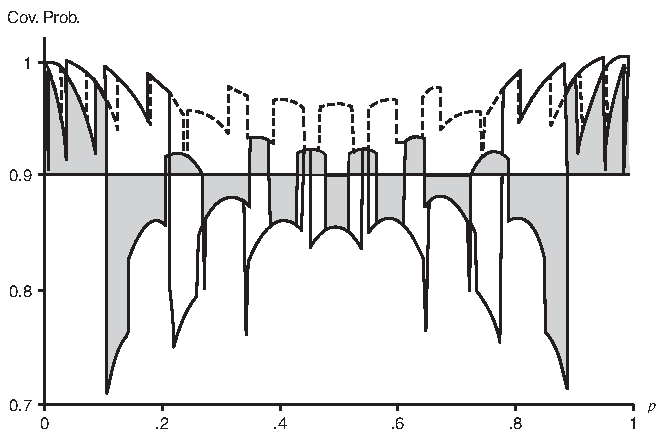
\includegraphics[width=.9\textwidth]{assets/chapter10/fig-10.4.2.pdf}
\caption{二项比例的名义$.9$置信程序的覆盖概率：LRT程序（细实线，灰色阴影）、得分程序（虚线）和修正Wald程序（粗实线）.}\label{fig:10.4.2}
\end{figure}\par
$$\hat\theta_M\pm z_{\alpha/2}\sqrt{\frac{\operatorname{Var}(\hat\theta_M)}n},$$
其中$\operatorname{Var}(\hat\theta_M)$由\eqref{eq:10.3.7}给出. 现在用估计\eqref{eq:10.3.8}与\eqref{eq:10.3.9}替换$\operatorname{Var}(\hat\theta_M)$，得到Wald型区间. 为评价它们，制作与\autoref{tab:10.4.7}相似的表. 有趣的是，除双指数分布外，\autoref{tab:10.4.8}中的区间表现都不如\autoref{tab:10.4.7}中基于通常均值与方差的区间. 对此没有很好的解释，只能再次归咎于$z_{\alpha/2}$临界值过于乐观.
\end{example}

\par\begin{table}[htbp]\centering
\caption{基于Huber $M$估计量、名义$1-\alpha=.9$的区间置信系数；$n=15$，基于10,000次模拟.}\label{tab:10.4.8}
\begin{tabular}{l|rrrr}\toprule
&\multicolumn{4}{c}{基础pdf}\\\cmidrule(lr){2-5}
名义水平&正态&$t_5$&逻辑斯蒂&双指数\\\midrule
方差估计\eqref{eq:10.3.8}&.844&.856&.855&.889\\
方差估计\eqref{eq:10.3.9}&.837&.867&.855&.910\\\bottomrule
\end{tabular}
\end{table}\par

迄今提到的近似都基于令$n\to\infty$. 不过，还有其他适合使用近似区间的情形. 在\autoref{ex:9.2.17}中，需要参数趋于无穷时的近似. 另一种情形见\autoref{ex:2.3.13}：对某些参数配置，泊松分布可以近似二项分布. 这提示，如果认为这种参数配置很可能成立，就能以泊松分布为基础构造近似二项区间. 本着这种想法，介绍下面这个略不寻常的例子.

\sourcepageanchor{439}
\begin{example}[负二项区间]\label{ex:10.4.9}\index{SI0140@负二项}
设$X_1,\ldots,X_n$独立同分布于negative binomial$(r,p)$. 假设$r$已知，希望得到$p$的置信区间. 利用$Y=\sum X_i\sim\operatorname{negative\ binomial}(nr,p)$，可以用多种方法构造区间. 利用二项分布与$F$分布关系的一个变形，可构造精确置信区间（\autoref{exercise:9.22}），也可使用正态近似（\autoref{exercise:10.41}）. 还有另一种近似，不依赖$n$大，而依赖$p$小.

\autoref{exercise:2.38}证明，当$p\to0$时，
$$2pY\longrightarrow\chi_{2nr}^2\quad\text{依分布}.$$
所以，对小$p$，$2pY$是枢轴量！据此可构造适用于小$p$的枢轴$1-\alpha$置信区间：
$$\left\{p:\frac{\chi_{2nr,1-\alpha/2}^2}{2y}\leq p\leq\frac{\chi_{2nr,\alpha/2}^2}{2y}\right\}.$$
细节见\autoref{exercise:10.47}.
\end{example}
